\subsection{Parámetros de la ecuación de estado cúbica}


Existen dos formas para calcular los parámetros de la ecuación dependiendo de la cantidad de compuestos presentes en el sistema a estudiar.
\begin{itemize}
 \item Compuesto puro
 \item Mezcla. 
\end{itemize}

La clase "Substance" realiza los cálculos para los compuestos puros, mientras que la clase "Mixture" realiza los cálculos para la mezcla. Una vez obtenido el cálculo de los parámetros la super clase "Homogeneous" utiliza los parámetros para realizar el cálculo de propiedades.

\begin{lstlisting}[caption=Cualquier objeto tipo Homogeneous puede calcular los parámetrod de la ecuación de estado cúbica a y b]
	Homogeneous system = ....
	double a = system.calculate_a_cubicParameter();
	double b = system.calculate_b_cubicParameter();
\end{lstlisting}


La estructura de la librería se muestra en \ref{fig:homogeneousCalculations}

\begin{figure}[!h]
  
  \centering
    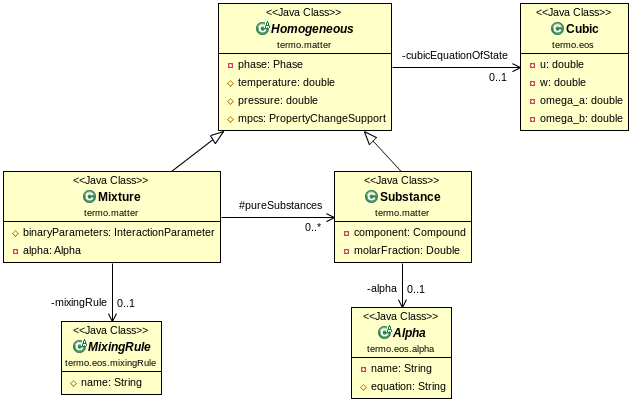
\includegraphics[scale=0.7]{homogeneousCalculations.png}
    \caption{A picture of a gull.}
    \label{fig:homogeneousCalculations}
\end{figure}

\subsection{Compuesto puro}
Los parámetros para un compuesto puro dependen de la ecuación de estado cúbica y de una expresión $\alpha$ .

\begin{equation}
	b_i = \Omega_b \frac{R T_{ci}}{p_{ci}} 
\end{equation}

\begin{equation}
 a_i = \Omega_a \frac{\left(R T_{ci}\right)^2}{p_{ci}} \alpha_i
\end{equation}

La expresión de $\alpha$ puede ser una función de la temperatura.

\begin{table}
\begin{tabular}{|c |c|c| }
	\hline
	Expresión & Parámetros & Ecuación de estado\\
	\hline
	Soave    &  ---& PR\\
	Peng and Robinson & ---& PR \\
	Mathias & $A$ & SRK\\
	Stryjek and Vera & $k_1$ & PRSV\\
	Adachi and Lu & $A,B$&SRK,PR\\
	Soave & $A,B$&SRK,PR\\
	Melhem, et al. & $A,B$&SRK,PR\\
	Androulakis et al. & $A,B,C$& SRK,PR\\
	Mathias and Copeman & $A,B,C$& SRK,PR\\
	Yu and Lu & $A,B,C$&SRK,PR\\
	Stryjek and Vera & $A,B,C$&PR\\
	Twu & $L,M,N$&TST\\
	Twu & ---&TST,PR\\
	GCEOS & ---& (Cualquier u y w)\\
	\hline
\end{tabular}
\caption{Expresiónes de $\alpha$ disponibles en la librería}\label{tab:alphas}
\end{table}


Para realizar el cálculo de los parámetros de la ecuación para el compuesto i, es necesario elegir la ecuación de estado cúbica (u,w, $\Omega_a$ y $\Omega_b$) y la expresión de $\alpha$.

En la sección \ref{subsec:pressure} se mostró como crear una ecuación de estado cúbica y asignar las variables $u$ y $w$. De igual manera podemos asignar el valor de $\Omega_a$ y $\Omega_b$ \footnote{Los valore de $\Omega_a$ y $\Omega_b$ se muestran en la tabla \ref{tab:cubics}}, o elegir la ecuación de estado cúbica previamente definida, a través de la clase ``EquatiosOfState''. Por comodidad usaremos la segunda aproximación.

Se debe elegir la expresión de $\alpha$ de la clase Alphas \footnote{Las expresiones de $\alpha$ disponibles se listan en \ref{tab:alphas}}. Es posible crear o modificar una expresión de $\alpha$, pero debido a su complejidad sera tratado en una sección aparte.

Para realizar el cálculo es necesario definir las propiedades del compuesto, temperatura crítica, presión crítica, y algunas expresiones de $\alpha$ necesitan el factor acéntrico, para lo cual existe la clase Compound que encapsula todas las propiedades del compuesto.



\begin{lstlisting}[caption=Cálculo de los parámetros de la ecuación de estado Soave Redlich Kwong y la expresión de $\alpha$ de mathias para el compuesto ]
import.termo.eos.Cubic;
...
Compound compound = new Compound("Cyclohexane");
compound.setCriticalPressure(4073000);
compound.setCriticalTemperature(553.5);
compound.setAcentricFactor(0.211);

Cubic srk = EquationsOfState.redlichKwongSoave();
Alpha mathias = Alphas.getMathiasExpression();

Substance substance = new Substance(srk,mathias, compound,Phase.LIQUID);

double a = substance.calculate_a_cubicParameter();
double b = substance.calculate_b_cubicParameter();
\end{lstlisting}





\subsubsection{Mezcla}

El cálculo de los parámetros para una mezcla depende de la regla de mezclado.Para las reglas de mezclado basadas en la energía libre de Gibbs de exceso el cálculo también depende del modelo de actividad elegido.

\begin{tabularx}{\textwidth}{|X|X|X|}
	\hline
	Regla & Parámetros & \\
	\hline
	Van Der Waals & $k_{ij}$ & $k_{ij} = k_{ji}$ \\
	Mathias-Klotz-Prausnitz& $k_{ij}$ & $k_{ij} \neq k_{ji}$ \\
	Basadas en la energía libre de Gibbs de exceso. & Segun el modelo de actividad y la implementación de la regla.& --- \\
	\hline
\end{tabularx}

Se necesita definir el conjunto de compuestos de la mezcla.

\begin{lstlisting}[caption=Cálculo de los parámetros de la ecuación de estado Soave Redlich Kwong y la expresión de $\alpha$ de mathias para el compuesto ]
import termo.component.Compound;
import termo.eos.Cubic;
import termo.eos.EquationsOfState;
import termo.eos.alpha.Alpha;
import termo.eos.alpha.Alphas;
import termo.matter.Mixture;
import termo.matter.Substance;
import termo.matter.factory.MixtureBuilder;
import termo.phase.Phase;
...
Compound cyclohexane = new Compound("Cyclohexane");
		cyclohexane.setCriticalPressure(4073000);
		cyclohexane.setCriticalTemperature(553.5);
		cyclohexane.setAcentricFactor(0.211);
		
		Compound pentane = new Compound("N-pentane");
		pentane.setCriticalPressure(3370000);
		pentane.setCriticalTemperature(469.7);
		pentane.setAcentricFactor(0.251);
		
		Cubic equationOfState = EquationsOfState.pengRobinson();
		Alpha alpha = Alphas.getMathiasAndCopemanExpression();
		
		Mixture mixture = new MixtureBuilder()
					.addCompounds(cyclohexane,pentane)
					.setAlpha(alpha)
					.setEquationOfState(equationOfState)
					.setPhase(Phase.VAPOR)
					.build();

		double a = mixture.calculate_a_cubicParameter();
		double b = mixture.calculate_b_cubicParameter();
\end{lstlisting}
